\section{Important results in finite dimensions}

\subsection{Implicit function theorem}

\begin{frame}{What is implicit function?}
    If a function is written in the form of
    \begin{equation}
        y = f(x), \text{ e.g., } y = 2x^3
    \end{equation}
    is called an \textbf{explicit function}. 
    \\And sometimes functions are given in the form 
    \begin{equation}
        y - f(x) = 0 \text{ e.g., } y - 2x^3 = 0
    \end{equation}
    is called an \textbf{implicit function}.\\
    In general, \textbf{implicit function} are written in a general form as
    \begin{equation}
        F(y, x) = 0
    \end{equation}
    \footnotetext[1]{While we can always change an explicit function into an implicit function (by taking $f(x)$ to the other side of the equality) the reverse is not always true}
\end{frame}

\begin{frame}{Motivation}
    \begin{parchment}[Question]
        \begin{enumerate}
            \item Given a solution to a system of equations, are there other solutions nearby? \\=> The analytic version of the implicit function theorem.
            \item What does the set of all solutions look like near a given solution? \\=> The geometric version of the implicit function theorem.
        \end{enumerate}
    \end{parchment}
\end{frame}

\begin{frame}{Implicit function theorem}
    \begin{block}{Theorem: Implicit function theorem}
        Suppose that $U \subseteq \R^n$, and $V \subseteq \R^m$ are open sets, and $\mathbf{F}: U \times V \rightarrow \R^m$ is a function of class $C^1$. Let $(x_0, y_0) \in U \times V$ is a point such that $\mathbf{F}(x_0, y_0) = 0$ and $D_y\mathbf{F}(x_0, y_0) : \R^m \rightarrow \R^m$, the derivative of $\mathbf{F}$ w.r.t $y$, is nonsingular, i.e $D_y\mathbf{F}(x_0, y_0) \ne 0$. Then
        \begin{itemize}
            \item There exists neighborhoods $U_1 \ni x_0$ and $V_1 \ni y_0$ and a $C^1$ mapping $y: U_1 \rightarrow V_1$ such that a point $(x, y) \in U_1 \times V_1$ satisfies $\mathbf{F}(x, y) = 0$ if and only if $y = \mathbf{f}(x)$. The derivative of $y$ at $x_0$ is given by
            \begin{equation}
                D_y(x_0) = -D_y\mathbf{F}(x_0, y_0)^{-1}D_x\mathbf{F}(x_0, y_0)
            \end{equation}
            \item Moreover, if $\mathbf{F}$ is $k$-times continously differentiable, i.e., $\mathbf{F} \in C^k$, then $\mathbf{f}(x) \in C^k$.
        \end{itemize}
    \end{block}
\end{frame}

\begin{frame}{Proof of Implicit function theorem}
    At first, we need to setup something...\\
    \vspace{1cm}
    If necessary, considering the function
    \begin{equation}
        (x,y) \mapsto f(x + x_0, y+ y_0) - f(x_0, y_0)
    \end{equation}
    And, let 
    \begin{equation}
        f(x) = (f_1(x, y), \dots, f_m(x, y))
    \end{equation}
\end{frame}

\begin{frame}{Proof of Implicit function theorem}
    $Df$ is continous $\Rightarrow$ exist neighborhoods $U_0 \in \R^n$, $V_0 \in \R^m$ that
    \begin{equation}
        \begin{bmatrix}
        \nabla_yf_1(x, y_1)^{\top}\\ 
        \nabla_yf_2(x, y_2)^{\top}\\ 
        \vdots\\ 
        \nabla_yf_m(x, y_m)^{\top}
        \end{bmatrix}
    \end{equation}
    is invertible for all $(x, y_i) \in U_0 \times V_0$.
\end{frame}

\begin{frame}{Proof of Implicit function theorem}
    \textbf{Question}: Is every $x \in U_0$, then there exists at most one $y \in V_0$ such that $f(x, y) = 0$.
    \vspace{0.5cm}
    By contradiction, suppose that $\exists y, z \in V_0, y \ne z, f(x,y) = f(x,z) = 0$. Due the mean value theorem, $\exists y_i \in (y, z)$ that
    \begin{equation}
        f_i(x,z) - f_i(x,y) = \left \langle \nabla_yf_i(x,y_i), z -y \right \rangle
    \end{equation}
    And the previous matrix is non-singular, so $y = z$.
\end{frame}

\begin{frame}{Proof of Implicit function theorem}
    Let $\overline{B}_r(0) \subseteq V_0$
    \begin{itemize}
        \item $f(0, y) \ne 0, \forall y \in S_r(0) := \{y \in \R^l : \left \| y \right \| = r\}$ due to $f(0,0) = 0$.
        \item $\exists \alpha > 0, \left \| f(0, y) \geq \alpha \right \|, \forall y \in S_r(0)$ due to $f$ is continous.
    \end{itemize}
\end{frame}

\begin{frame}{Proof of Implicit function theorem}
    Consider the function 
    \begin{equation}
        F(x, y) := \left \| f(x, y) \right \|^2 = \sum_{i=1}^mf_i(x, y)^2
    \end{equation}
    that satisfies the properties 
    \begin{itemize}
        \item $F(0, y) \geq \alpha > 0, \forall y \in S_r(0)$
        \item $F(0, 0) = 0$
    \end{itemize}
\end{frame}

\begin{frame}{Proof of Implicit function theorem}
    Because $F$ is continous function, $\exists U_1 \subseteq U_0$ of $0 \in \R^n$ such that
    \begin{equation}
        F(x,y) \geq \frac{\alpha}{2}, F(x, 0) \leq \frac{\alpha}{2} \forall x \in U_1, y \in S_r(0)
    \end{equation}
    fixed $x \in U_1$, function $y \mapsto F(x, y)$ achieves its minimum on $\overline{B}_r(0)$ at $y(x)$ in the interior of $\overline{B}_r(0)$
    \begin{equation}
        D_yF(x,y(x)) = 2D_yf(x, y(x))f(x,y(x)) = 0
    \end{equation}
    And the matrix $D_yf(x, y(x))$ is non-singular, so that
    \begin{equation}
        f(x,y(x)) = 0
    \end{equation}
\end{frame}

\begin{frame}{Proof of Implicit function theorem}
    Writting $\Delta y := y(x+\Delta x) - y(y)$, by the mean value theorem
    \begin{equation}
        0 = D_xf(\widetilde{x}, \widetilde{y})\Delta x + D_yf(\widetilde{x}, \widetilde{y})\Delta y
    \end{equation}
    for some point $(\widetilde{x}, \widetilde{y})$ one the line segment between $(x, y(x))$ and $(x + \Delta x, y(x + \Delta x))$. And as $\left \| \Delta x \right \| \rightarrow 0$,  $\left \| \Delta y \right \| \rightarrow 0$, thus lead $y(x)$ is continous.
    \vspace{1cm}
    And by Taylors formula and continuity of $y(x)$, we prove that $y(x)$ is Fréchet differentiable.
    \vspace{1cm}
    If $f \in C^2$, then $y(x) \in C^2$. And in general, if $C^k$, we prove by induction on $k$ that $y(x)$ is $C^k$.
\end{frame}

\begin{frame}{Discussion about the analytic meaning}
    \begin{parchment}[Problem]
        Solving the equation below:
        \begin{equation}
            f(x, y) = 0
        \end{equation}
        for $y$ as a function of $x$, and say $y = f(x)$
    \end{parchment}
    If we have a solution $b = f(a)$, then in principle it is possible to solve for $x$ near $a$, if the crucial hypothesis $D_yf(a, b) \ne 0$ holds.\\
    In this meaning, Implicit function theorem is a theorem about the \textbf{possibility of solving a system of nonlinear equations}.
\end{frame}

\begin{frame}{Discussion about the geometric meaning}
    There are 3 natural ways to represent a curve $S \subseteq \R^n$
    \begin{itemize}
        \item As a graph
        \item As a level set
        \item Parametrically
    \end{itemize}
\end{frame}

\begin{frame}{Discussion about the geometric meaning}
    Considering the case $n = 2$
    \begin{itemize}
        \item Graph: \begin{equation}
        \left. 
        \begin{array}{c}
        S = \{ (x,y) \in \R^2:  \ y = f(x) \text{ for }x\in I\}\\
        \text{OR} \\
        S = \{ (x,y) \in \R^2:  \ x = f(y) \text{ for }y\in I\}
        \end{array}\right\}
        \label{graph}
        \end{equation}
        for some $f:I\to \R$, where $I\subseteq \R$ is an interval.
        \item Level set, is, a set of the form
        \begin{equation}
            S    = \{ (x,y)\in U : F(x,y) = c \} 
        \label{locus}\end{equation}
        for some open $U\subseteq \R^2$, some $F:U\to \R$, some $c\in \R$.
        \item Parametrically, in the form
        \begin{equation}
        S    = \{  \mathbf f(t) :  \ t\in I \} 
        \label{parametrically}\end{equation}
        for some interval $I\subseteq \R$, and some $\mathbf f:I\to \R^2$
    \end{itemize}
\end{frame}

\begin{frame}{Discussion about the geometric meaning}
    \begin{figure}[h!]
        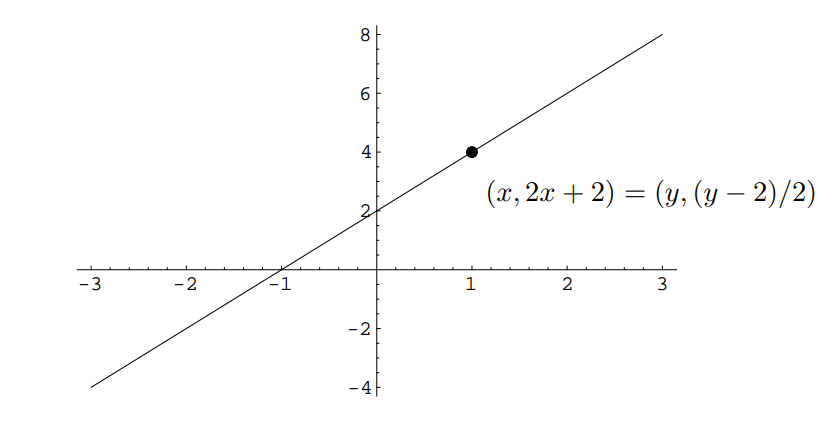
\includegraphics[width=0.75\linewidth]{figures/implicit_function_example01.png}
        \caption{The line $2x − y + 2 = 0$ as the graph of $f(x) = 2x + 2$ or of $g(y) = (y − 2)/2$}
    \end{figure}
\end{frame}

\begin{frame}{Discussion about the geometric meaning}
    \begin{figure}[h!]
        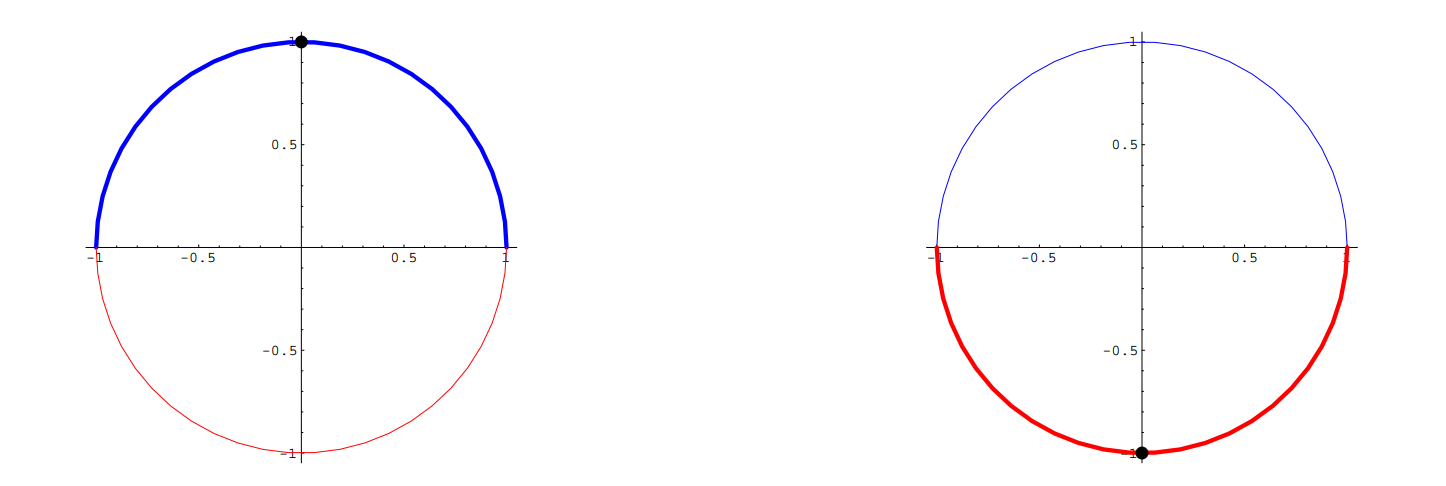
\includegraphics[width=0.75\linewidth]{figures/implicit_function_example02.png}
        \caption{The thick arcs are the graphs of $x \mapsto \pm \sqrt{1-x^2}$}
    \end{figure}
\end{frame}

\begin{frame}{Discussion about the geometric meaning}
    \begin{figure}[h!]
        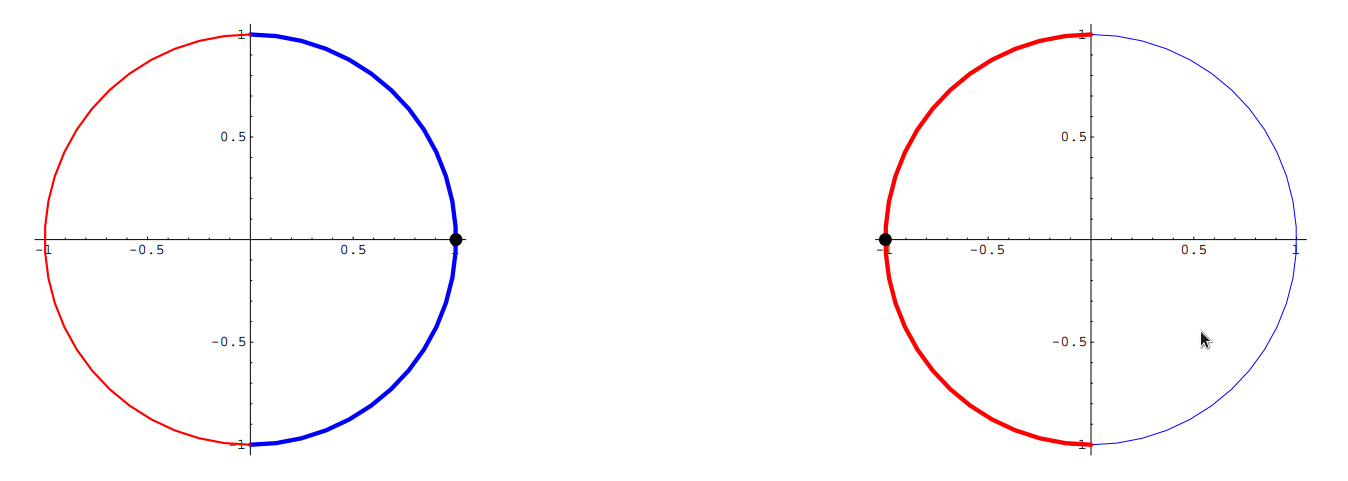
\includegraphics[width=0.75\linewidth]{figures/implicit_function_example03.png}
        \caption{The thick arcs are the graphs of $y \mapsto \pm \sqrt{1-y^2}$}
    \end{figure}
\end{frame}

\begin{frame}{Discussion about the geometric meaning}
    \begin{figure}[h!]
        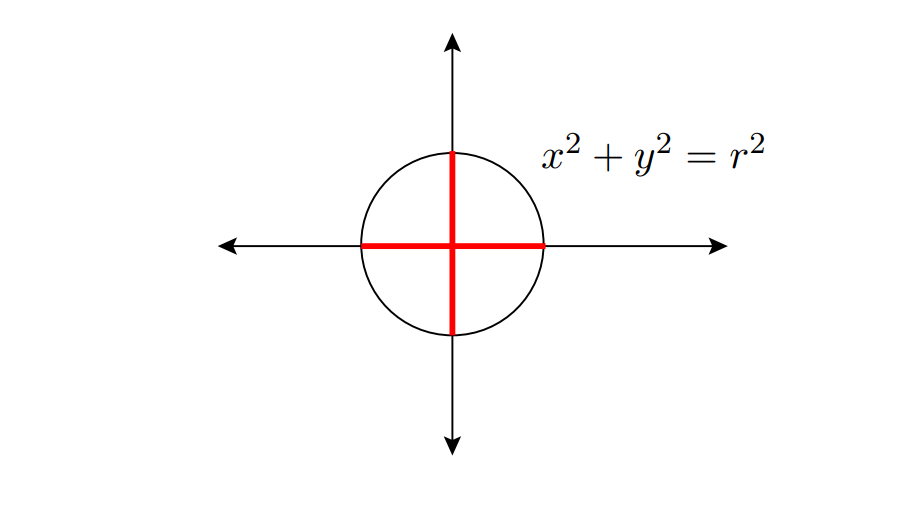
\includegraphics[width=0.75\linewidth]{figures/implicit_function_example04.png}
        \caption{Can the thick line segments be a graph?}
    \end{figure}
\end{frame}


\begin{frame}{Why the Implicit Function Theorem is a great theorem?}
    \begin{parchment}[Fact]
        With given $k$ \text{nonlinear equations} in $k$ unknowns:
        \begin{itemize}
            \item It is \textbf{impossible to solve}.
            \item It is often \textbf{impossible to determine whether it has any solutions}.
        \end{itemize}
    \end{parchment}
    The Implicit Function Theorem allows us to (partly) reduce impossible questions about systems of nonlinear equations to straightforward questions about systems of linear equations. 
\end{frame}

% \begin{frame}{Limitation of the Implicit Function Theorem}
%     Some limitation of the Implicit Function Theorem
%     \begin{itemize}
%         \item 
%     \end{itemize}
% \end{frame}

\begin{frame}{Some special cases of the implicit function theorem}
    \begin{block}{Theorem: Implicit function theorem, $m=n=1$}
        Suppose that $F$ is real-valued $C^1$ function defined for all $(x, y)$ in open set $U\times V \subseteq \R^2$.
        \begin{itemize}
            \item If $f(a, b) = 0$ and $\partial_yf(a, b) \ne 0$, then the equation
            \begin{equation}
                F(x, y) = 0
            \end{equation}
            implicitly determines $y$ as a $C^1$ function of $x$, i.e., $y = f(x)$, for $x$ near $a$.  Moreover $f(a) = b$.
            \item If $f(a, b) = 0$ and $\partial_xf(a, b) \ne 0$, then the equation
            \begin{equation}
                F(x, y) = 0
            \end{equation}
            implicitly determines $x$ as a $C^1$ function of x, i.e., $x = f(y)$, for $y$ near $b$.  Moreover $f(b) = a$.
        \end{itemize}
    \end{block}
\end{frame}

\begin{frame}{Some special cases of the implicit function theorem}
    \begin{block}{Theorem: Implicit function theorem, $n=2, m=1$}
    Suppose that $F$ is a scalar function of class $C^1$ function defined for all $(x, y, z)$ in open set $U\times V \subseteq \R^3$.
    \begin{itemize}
        \item If $f(a, b, c) = 0$ and $\partial_zf(a, b, c) \ne 0$, then the equation
            \begin{equation}
                F(x, y, x) = 0
            \end{equation}
            implicitly determines $z$ as a $C^1$ function of $(x, z)$, i.e., $z = f(x, y)$ for $(x, y)$ near $(a, b)$. Moreover, $f(a, b) = c$.
        \item Similarly, we also have results in the cases: $f(a, b, c) = 0$ and $\partial_yf(a, b, c) \ne 0$; and $f(a, b, c) = 0$ and $\partial_xf(a, b, c) \ne 0$
    \end{itemize}
    \end{block}
\end{frame}

\begin{frame}{Some special cases of the implicit function theorem}
    \begin{block}{Theorem: Implicit function theorem, $n=1, m=2$}
    Suppose that $\mathbf{F} = (F_1, F_2)$ is function $U \times V \rightarrow \R^2$ of class $C^1$ defined for all $(x, y, z)$ in open set $U\times V \subseteq \R^3$.
    \begin{itemize}
        \item If $\mathbf{F}(a, b, c) = \mathbf{0}$ and 
        \begin{equation}
            \begin{vmatrix}
             \partial_yF_1 & \partial_zF_1\\ 
             \partial_yF_2 & \partial_zF_2
            \end{vmatrix} \ne 0
        \end{equation} 
        then
        \begin{equation}
            \mathbf{F}(x, y, z) = \mathbf{0} \Leftrightarrow \begin{cases}
                F_1(x, y, z) = 0\\
                F_2(x, y, z) = 0\\
            \end{cases}
        \end{equation}
        implicitly determines $(y, z)$ as a $C^1$ function of $x$, i.e., $(y, z) = \mathbf{f}(x)$, for $x$ near $a$. Moreover, $\mathbf{f}(b, c) = f(a)$.
        \item Similarly, we also have results in the remain cases.
    \end{itemize}
    \end{block}
\end{frame}

\begin{frame}{Computational example 1}
    % \begin{parchment}[Problem 01]
    %     Considering the general $F: \R^3 \rightarrow \R$ of class $C^1$. Suppose that at a point $(a,b,c)\in \R^3$, we have $F(a,b,c) = 0, \partial_z F(a,b,c)\ne 0$. Does the equation implicitly determine $z$ as a function $f(x, y)$ for $(x,y)$ near $(a, b)$ with $f(a, b) = c$? If so, find a formula for $\partial_x f(x,y)$, and evaluate it at $(x, y) = (a, b)$.
    % \end{parchment}
    \begin{parchment}[Problem 01]
        Consider the equation
        \begin{equation}
            F(x,y,z) = xy+ xz \ln(yz)  =1
        \end{equation}
        We know that $(1, 1, 1)$ is a solution. Does the equation implicitly determine $z$ as a function $f(x, y)$ for $(x,y)$ near $(1, 1)$ with $f(1, 1) = 1$? If so, find a formula for $\partial_x f(1, 1)$, and evaluate it at $(1, 1) = (1, 1)$.
    \end{parchment}
\end{frame}

\begin{frame}{Computational example 1}
    We have
    \begin{equation}
        \partial_zF = xln(yz) + x
    \end{equation}
    And at $(x, y, z) = (1, 1, 1)$, $F(1, 1, 1) = 1$. So the Implicit Function Theorem guarantees that there is a function $f(x, y)$, defined for $(x, y)$ near $(1, 1)$ such that
    \begin{equation}
        F(x, y,z) = 1 \text{ when } z = f(x, y)
    \end{equation}
    To find $\partial_xf$, by using the original equation that defines $z$ as a function of $(x, y)$ to differentiate both sides with respect to $x$.
    \begin{equation}
        y + zln(yz) + x\dfrac{\partial z}{\partial x}ln(yz) + \dfrac{xz}{yz}y\dfrac{\partial z}{\partial x} = 0 \Leftrightarrow \dfrac{\partial z}{\partial x} = - \dfrac{y + zln(yz)}{x + xln(yz)}
    \end{equation}
    Evaluating at $(x, y, z) = (1, 1, 1)$, and solving for $\dfrac{\partial z}{\partial x}$. We have:
    \begin{equation}
        1 + \dfrac{\partial z}{\partial x} = 0 \Leftrightarrow \dfrac{\partial z}{\partial x} = -1
    \end{equation}
\end{frame}

\begin{frame}{Computational example 2}
    \begin{parchment}[Problem 02]
        Consider the system of equations
        \begin{align}
            F_1(x,y,u,v) = xye^u +  \sin(v-u) &= 0\\\
            F_2(x,y,u,v)  =(x+1)(y+2)(u+3)(v+4) - 24 &=0
        \end{align}
        We know that $(0, 0, 0, 0)$ is a solution. Does the system of equations implicitly determine $(u, v$ as a function of $(x, y)$, i.e., $(u,v) = \mathbf{f}(x, y)$ for $(x, y)$ near $(0, 0)$? If so, find a formula for $\partial_x \mathbf{f}(x, y)$ at $(x, y) = (0, 0)$ 
    \end{parchment}
\end{frame}

\begin{frame}{Computational example 2}
    Let $\mathbf F = \binom{F_1}{F_2}$. Then
    \begin{equation}
        \left(\begin{array}{ll}
        \partial_u F_1&\partial_v F_1\\\
        \partial_u F_2&\partial_v F_2
        \end{array}
        \right)  \ = \ 
        \left(\begin{array}{cc}
        xye^u  - \cos(v-u)&\cos(v-u)\\\
        (x+1)(y+2)(v+4)&(x+1)(y+2)(u+3)
        \end{array}
        \right)
    \end{equation}
    At $(x,y,u,v) = (0,0,0,0)$,
    \begin{equation}
        \left(\begin{array}{ll}
        \partial_u F_1(0,0,0,0)&\partial_v F_1(0,0,0,0)\\\
        \partial_u F_2(0,0,0,0)&\partial_v F_2(0,0,0,0)
        \end{array}\right)
        = \left(\begin{array}{rr}
        -1&1\\ 8&6
        \end{array}
        \right)
    \end{equation}
    This matrix is invertible, so the theorem guarantees that the equations implicitly determine $(u, v)$ as a function of $(x, y)$
\end{frame}

\begin{frame}{Computational example 2}
    Find $\partial_x \mathbf f = \binom{\partial_x f_1}{\partial_x f_2}$, where $\binom uv = \mathbf f(x,y) = \binom{f_1(x,y)}{f_2(x,y)}$. Considering equations below:
    \begin{align}
        \begin{aligned}
            xye^u +  \sin(v-u) &= 0\\\
            (x+1)(y+2)(u+3)(v+4) - 24 &=0.
        \end{aligned}
    \end{align}
    and differentiate everything with respect to $x$:
    \begin{align}
        \begin{aligned}
            ye^u + \left( xy e^u - \cos(v-u)\right) \frac{\partial u}{\partial x} + \cos(v-u)\frac{\partial v}{\partial x} &= 0\\\
            (y+2)(u+3)(v+4) +(x+1)(y+2)(v+4)\frac{\partial u}{\partial x} +(x+1)(y+2)(u+3)\frac{\partial v}{\partial x}   &=0.
        \end{aligned}
    \end{align}
\end{frame}

\begin{frame}{Computational example 2}
    At $(x,y,u,v) = (0,0,0,0)$,
    \begin{align}
    \left(\begin{array}{rr}
    -1&1\\\ 8&6
    \end{array}
    \right)\binom
    {\frac{\partial u}{\partial x}}
    {\frac{\partial v}{\partial x}} = \binom 0{-24}.
    \label{concrete}\end{align}
    And
    \begin{equation}
            \binom{\frac{\partial u}{\partial x}}
{\frac{\partial v}{\partial x}} = \frac{1}{-14}
\left(
\begin{array}{rr}
6&-1 \\\
-8&-1
\end{array}
\right)\binom0 {-24} =  -\binom{12/7}{12/7}.
    \end{equation}
\end{frame}

\subsection{Inverse function theorem}

\begin{frame}{What is Transformations?}
    \begin{parchment}{Fact}
        Let $U$, and $V$ be two open subsets of $\R^n$. Considering functions as
        \begin{equation}
            \mathbf{f}: U \rightarrow V
        \end{equation}
        is called \emph{transformation}. \\
        If $\mathbf{f}$ is a bijection (that is, both one-to-one and onto). Then implies that $\mathbf{f}^{-1}: V \rightarrow U$ exists. And both $\mathbf{f}$, $\mathbf{f}^{-1}$ are class of $C^1$.
    \end{parchment}
    
\end{frame}

\begin{frame}{Example}
    Considering the transformation of Cartesian grid by using the linear mapping $\mathbf f(x,y) = (2y-x,x+y)$.
    \begin{columns}
        \begin{column}{0.5\textwidth}
            \begin{figure}[h!]
                
\includegraphics[width=0.95\linewidth]{figures/Grid.jpg}
                \caption{Before transformation.}
                \label{fig:example-astatic-knowledge-graph}
            \end{figure}
        \end{column}
        \begin{column}{0.5\textwidth}  %%<--- here
            \begin{figure}[h!]
                
\includegraphics[width=0.95\linewidth]{figures/linear_after.jpg}
                \caption{After transformation.}
                \label{fig:example-astatic-knowledge-graph}
            \end{figure}
        \end{column}
    \end{columns}
\end{frame}

\begin{frame}{The Inverse Function Theorem}
    \begin{block}{Theorem: The Inverse Function Theorem}
        Let $\mathbf{f}$ be a $C^1$ map from a neighborhood of $x_0 \in \R^n$ into $\R^n$. If $D\mathbf{f}(x_0)$ is non-singular, then there exist neighborhoods $U \ni x_0$ and $V \ni y_0 = \mathbf{f}(x_0)$ such that $ \mathbf{f} : U \rightarrow V$ is a $C^1$ diffeomorphism\footnotemark, and 
        \begin{equation}
            D\mathbf{f}^{-1}(y) = D\mathbf{f}(x)^{-1} \text{ for all} (x, y) \in U \times V, y = \mathbf{f}(x)
        \end{equation}
        Moreover, if $\mathbf{f}$ is $C^k$, then $\mathbf{f}$ is a $C^k$ diffeomorphism on $U$.
    \end{block}
    \footnotetext{A diffeomorphism is an isomorphism of smooth manifolds. It is an invertible function that maps one differentiable manifold to another such that both the function and its inverse are continuously differentiable.}
\end{frame}

\begin{frame}{Proof of The Inverse Function Theorem}
    We can define the function 
    \begin{equation}
        F(x, y) = f(x) - y
    \end{equation}
    and, find that
    \begin{equation}
        D_xF(x_0, y) = Df(x_0)
    \end{equation}
    is non-singular.
    \vspace{1cm}
    And apply the Implicit function theorem to $F$.
\end{frame}

\begin{frame}{The usage of Implicit Function Theorem}
    \begin{parchment}{Problem}
        Suppose that given $\mathbf{f}: U \rightarrow V$, and $\mathbf{y}  \in V$, find $\mathbf{x}$ by solving 
        \begin{equation}
            \mathbf{f}(\mathbf{x}) = \mathbf{y}
        \end{equation}
    \end{parchment}
    \begin{parchment}{Fact}
        This problem is often an impossible problem to solve handle.
    \end{parchment}
    
\end{frame}
\begin{frame}{The usage of Implicit Function Theorem}
    \begin{parchment}[The Inverse Function Theorem says]
        If we know that $\mathbf{f}(\mathbf{a}) = \mathbf{b}$, then for $\mathbf{y}$ near $\mathbf{b}$, the solvability of the \textbf{nonlinear system} can be established by considering a \textbf{much easier} question about linear algebra, whether the matrix $D\mathbf{f}(a)$ is invertible.
    \end{parchment}
\end{frame}

\begin{frame}{Computational example}
    \begin{parchment}[Problem 03]
       Determine whether the system
        \begin{equation}
            \begin{cases}
                u(x, y, z) = x + xyz\\
                v(x, y, z) = y + xy\\
                w(x, y, z) = z + 2x + 3z^2
            \end{cases}
        \end{equation}
        can be solved for $x, y, z$ in terms of $u, v, w$ near $p = (0, 0, 0)$.
    \end{parchment}
\end{frame}

\begin{frame}{Computational example}
    Let $\mathbf{F}(x, y,z) = (u, v, w)$, then
    \begin{equation}
        D\mathbf{F}(p) = \begin{pmatrix}
         u_x& u_y & u_z\\ 
         v_x& v_y & v_z\\ 
         w_x& w_y & w_z
        \end{pmatrix}(p)
        = \begin{pmatrix}
         1+yz& xz & xy\\ 
         y& 1+x & 0\\ 
         2& 0 & 1+6z
        \end{pmatrix}(p)
        = \begin{pmatrix}
         1& 0 & 0\\ 
         0& 1 & 0\\ 
         2& 0 & 1
        \end{pmatrix}
    \end{equation}
    Due to,
    \begin{equation}
        \begin{vmatrix}
         1& 0 & 0\\ 
         0& 1 & 0\\ 
         2& 0 & 1
        \end{vmatrix} = 1 \ne 0
    \end{equation}
    By the Inverse Function Theorem, the inverse function $F^{-1}(u,v,w)$ exists near $p=(0, 0,0)$, i.e., we can solved for $x, y, z$ in terms of $u, v, w$ near $p = (0, 0, 0)$.
\end{frame}

\subsection{Lyusternik theorem}

\begin{frame}{The Lyusternik theorem}
    \begin{block}{Definition of tangent direction}
        Let $M$ be a non-empty subset of $\R^n$ and $x \in M$. A vector $d \in R^n$ is called a tangent direction of $M$ at $x$ if there exist a sequence $x_n \in M$ converging to $x$ and a non-negative seqence $\alpha_n$ such that
        \begin{equation}
            \underset{n\rightarrow\infty}{\lim}\alpha_n(x_n-x)=d
        \end{equation}
        The tangent cone of $M$ at $x$, donated by $T_M(x)$, is the set of all tangent direction of $M$ at $x$.
    \end{block}
\end{frame}

\begin{frame}{The Lyusternik theorem}
    \begin{block}{Theorem: The Lyusternik theorem}
        Let $\mathbf{F}: U \rightarrow \R^m$ be $C^1$ map, where $U \subset \R^n$ be an open set. Let $M = \mathbf{F}^{-1}(\mathbf{F}(x_0))$ be the level set of a point $x_0 \in U$. If the derivative $D\mathbf{F}(x_0)$ is a linear map onto $\R^m$, then the tangent cone of $M$ is the null space of the linear map $D\mathbf{F}(x_0)$, that is,
        \begin{equation}
            T_M(x_0) = \{d \in \R^n: D\mathbf{F}(x_0)d=0\}
        \end{equation}
    \end{block}
\end{frame}

\begin{frame}{The proof of Lyusternik theorem}
    If nescessary, we will consider the function
    \begin{equation}
        x \mapsto f(x + x_0) - f(x_0)
    \end{equation}
    Assume that $x_0 = 0$, and $f(x_0) = 0$. And, define $A:= Df(0)$
\end{frame}

\begin{frame}{The proof of Lyusternik theorem}
    Now, we will prove that
    \begin{equation}
        T_M(0) \subseteq \text{Ker}A
    \end{equation}
    If $d \in T_M(0)$, then there exists points $x(t) = td + o(t) \in M$. We have:
    \begin{align}
        \begin{aligned}
            f(x) &=0\\
            f(x(t)) & = 0\\
            f(td + o(t) + 0) &= 0\\
            tDf(0)(d) + o(t) + f(0) &= 0\\
            Df(0)(d) + \frac{o(t)}{t} &= 0\\
            \lim_{t \rightarrow \infty}\left(Df(0)(d) + \frac{o(t)}{t}\right) &= 0\\
            Df(0)(d) &= 0
        \end{aligned}
    \end{align}
\end{frame}

\begin{frame}{The proof of Lyusternik theorem}
    Idea to prove the reverse inclusion: the equation $f(x) = 0$ can be written as $f(y,z) = 0$in a form that is suitable for applying the implicit function theorem.
\end{frame}

\begin{frame}{The proof of Lyusternik theorem}
    Define $K:= \text{Ker}A$, and $L := K^{\perp}$. Since $A:= Df(0)$ is onto $\R^m$, we can identify $K$ and $L$ with $\R6{n-m}$ and $\R^m$ respectively, by introducing a suitable basis in $\R^n$.\\
    For a point $x \in \R^n$ in form that $x = (y, z) \in K \times L$, we have $A = [D_yf(0), D_zf(0)]$, and
    \begin{equation}
        0 = A(K) = \{A(d_1, 0) : d_1 \in R^{n-m} = D_yf(0)(\R^{n-m}\}
    \end{equation}
    so that $D_yf(0) = 0$. And due to $A$ has rank $m$, so that $D_zf(0)$ is non-singular.
\end{frame}

\begin{frame}{The proof of Lyusternik theorem}
    Following the Implicit function theorem, there exists neighborhoods $U_1 \subseteq \R^m$, and $U_2 \subseteq \R^{n-m}$ around the origin and a $C^1$ map $\alpha: U_1 \rightarrow U_2, \alpha(0) = 0$, such that $x = (y, z) \in U_1 \times U_2$ satisfies $f(x) = 0$ if and only if $z = \alpha(y)$. The equation $f(x) = 0$ can be written as $f(y, \alpha(y))$. Differentiating this equation
    \begin{align}
        \begin{aligned}
            D_yf(y, \alpha(y)) + D_zf(y, \alpha(y)D_\alpha(y) = 0
        \end{aligned}
    \end{align}
    At $x = 0$, $D_yf(0) = 0$, and $D_zf(0)$ is non-singular, so that $D_\alpha(0) = 0$
\end{frame}

\begin{frame}{The proof of Lyusternik theorem}
    If $|y|$ is small:
    \begin{equation}
        \alpha(y) = \alpha(0) + D\alpha(0)y + o(y) = o(y)
    \end{equation}
    Let $d = (d_1, 0) \in K$, as $t \rightarrow 0$, the point $x(t) := (td_1, \alpha(td_1)) = (td_1, o(t))$ lies in $M$. And that is $f(x(t)) = 0$, and satisfies 
    \begin{equation}
        \frac{x(t) - td}{t} = \frac{(0, o(t))}{t} \rightarrow 0
    \end{equation}
    This implies that $K \subseteq T_M(0)$.
\end{frame}

\begin{frame}{The usage of the Lyusternik theorem}
    The usage of the Lyusternik theorem (finite version)
    \begin{itemize}
        \item Application in multi-objective optimization \cite{jimenez2002finite}
    \end{itemize}
\end{frame}